\chapter[Dạng bài: Tổng hợp các dao động cùng phương, cùng tần số]{Dạng bài: Tổng hợp các dao động cùng phương, cùng tần số}
\section{Lý thuyết}
\subsection{Biểu diễn dao động điều hòa bằng vectơ quay }
Một dao động điều hòa với phương trình 
$$x=A\cos(\omega t+\varphi)$$
có thể được biểu diễn bởi một vectơ $\overrightarrow{\textrm{OM}}$ quay đều với tốc độ góc $\omega$. Vectơ quay có những đặc điểm như sau:
\begin{itemize}
	\item Có gốc tại \bltext{gốc tọa độ} của trục $\textrm{O}x$; 
	\item Có độ dài bằng \bltext{biên độ dao động}, $\textrm{OM}=A$;
	\item Hợp với trục $\textrm{O}x$ một góc bằng \bltext{pha ban đầu $\varphi$} (chọn chiều dương là chiều dương của đường tròn lượng giác).
\end{itemize}
\begin{center}
	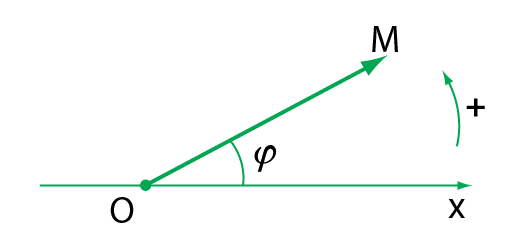
\includegraphics[width=0.5\textwidth]{../figs/VN12-PH-06-A-004-1-V2-01.png}
\end{center}

\subsection{Tổng hợp dao động bằng phương pháp giản đồ Fresnel} 
Do mỗi dao động có thể biểu diễn bằng một vectơ quay nên tổng hợp hai (hoặc nhiều) dao động có thể thực hiện bằng cách tính tổng vectơ của hai (hay nhiều) vectơ quay tương ứng.

Tổng hợp của hai dao động điều hòa cùng phương cùng tần số
\begin{eqnarray*}
	x_1&=&A_1\cos(\omega t+\varphi_1)\\
	x_2&=&A_2\cos(\omega t+\varphi_2)
\end{eqnarray*}	 
là một dao động \bltext{cùng} phương, \bltext{cùng} tần số, có phương trình 
$$x=x_1+x_2=A\cos(\omega t+\varphi),$$
trong đó:
\begin{itemize}
	\item Biên độ của dao động tổng hợp được tính như sau:
	\begin{equation*}\label{eq1}
		A^2=A^2_1+A^2_2 + 2A_1 A_2\cos(\varphi_2-\varphi_1), 
	\end{equation*}
	\item Pha ban đầu được tính bằng công thức:
	\begin{equation*}\label{eq2}
		\tan\varphi = 	\dfrac{A_1\sin\varphi_1+A_2\sin\varphi_2}		{A_1\cos\varphi_1+A_2\cos\varphi_2}. 
	\end{equation*}
\end{itemize}
\begin{center}
	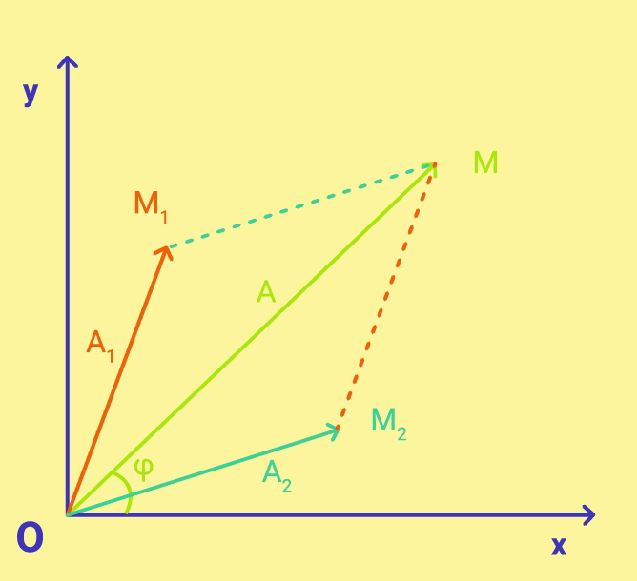
\includegraphics[width=0.4\textwidth]{../figs/VN12-PH-06-A-004-1-V2-02.jpg}
\end{center}

\subsection{Ảnh hưởng của độ lệch pha}

\begin{description}
	\item[Nếu các dao động thành phần cùng pha,] nghĩa là: 
	$$\Delta \varphi = \varphi_2-\varphi_2=2n\xsi{\pi}{\radian},\qquad \textrm{với } n=0,\pm 1, \pm 2, ...$$ thì biên độ dao động tổng hợp là  \bltext{\textbf{lớn nhất}}:$$A=A_1+A_2.$$ 
	
	\item [Nếu các dao động thành phần ngược pha,] nghĩa là: 
	$$\Delta \varphi = \varphi_2-\varphi_2=(2n+1)\xsi{\pi}{\radian} \qquad \textrm{với } n=0,\pm 1, \pm 2, ...$$ thì biên độ dao động tổng hợp là \bltext{\textbf{nhỏ nhất}}:$$A=\vert A_1-A_2\vert.$$
	
	\item [Nếu các dao động thành phần vuông pha,] nghĩa là: 
	$$\Delta \varphi = \varphi_2-\varphi_2=n\xsi{\pi}{\radian}+\dfrac{\pi}{2} \qquad \textrm{với } n=0,\pm 1, \pm 2, ...$$ thì biên độ dao động tổng hợp là: $$A^2=A^2_1+A^2_2.$$
	
\end{description}
\section{Mục tiêu bài học - Ví dụ minh họa}
\begin{dang}{Ghi nhớ được các công thức\\ tổng hợp dao động điều hòa}
	\viduii{1}{Ta có thể tổng hợp hai dao động thành phần khi hai dao động này
		\begin{mcq}
			\item cùng phương, cùng tần số.
			\item cùng biên độ và cùng tần số.
			\item cùng tần số và có độ lệch pha không đổi.
			\item cùng phương, cùng tần số và có độ lệch pha không đổi theo thời gian
			
		\end{mcq}
	}
	{\begin{center}
			\textbf{Hướng dẫn giải}
		\end{center}
		
		Ta chỉ có thể tổng hợp hai dao động khi hai dao động này có cùng phương cùng tần số và độ lệch pha không đổi theo thời gian.
		
		\textbf{Đáp án: D.}
	}
	\viduii{1}{Chọn phát biểu \textbf{sai}. Trong tổng hợp dao động, biên độ của dao động tổng hợp
		\begin{mcq}
			\item cực đại khi độ lệch pha giữa hai dao động thành phần là $2\pi$.
			\item cực tiểu khi độ lệch pha giữa hai dao động thành phần là $\pi$.
			\item phụ thuộc vào tần số của hai dao động thành phần.
			\item phụ thuộc và độ lệch pha giữa hai dao động thành phần.
		\end{mcq}
	}
	{\begin{center}
			\textbf{Hướng dẫn giải}
		\end{center}
		
		Biên độ dao động tổng hợp không phụ thuộc vào tần số của hai dao động thành phần.
		
		\textbf{Đáp án: C.}
	}
	
\end{dang}
\begin{dang}{Sử dụng được các công thức, liên hệ được phương trình dao động điều hòa\\ và số phức, tính biên độ, độ lệch pha\\ tổng hợp của các dao động}
	\ppgiai{\subsection{Phương pháp tổng hợp dao động bằng giản đồ Fresnel}
		
		Ta áp dụng công thức tính biên độ dao động tổng hợp là
		
		$$	A^2=A^2_1+A^2_2 + 2A_1 A_2\cos(\varphi_2-\varphi_1)$$ và pha ban đầu của dao động tổng hợp là
		
		$$\tan\varphi = 	\dfrac{A_1\sin\varphi_1+A_2\sin\varphi_2}		{A_1\cos\varphi_1+A_2\cos\varphi_2}$$.  
		
		\subsection{Phương pháp tổng hợp dao động bằng số phức}
		
		Đầu tiên, ta phải biết biểu diễn một dao động điều hòa sang số phức bằng máy tính cầm tay CAISO fx-580 VNX, tức là từ dạng $x=A\cos(\omega t+\varphi)\rightarrow A\angle \varphi$.
		
		\begin{description}
			\item[Bước 1] Thiết lập môi trường tính toán số phức với lệnh:
			\begin{center}
				
\includegraphics[width=0.5\textwidth]{../figs/VN12-PH-06-A-004-1-V2-03.jpg}
			\end{center}
			
			\item[Bước 2] Thiết lập số phức ở dạng lượng giác $A\angle \varphi$:
			\begin{center}
				
\includegraphics[width=0.5\textwidth]{../figs/VN12-PH-06-A-004-1-V2-04.jpg}
			\end{center}
			
			\item[Bước 3] Nhập số liệu theo yêu cầu đề bài.
			
			\luuy{Cài đặt góc dưới dạng radian (nếu cần).}
		\end{description}
	}
	\viduii{2}{ Một vật thực hiện đồng thời hai dao động điều hòa $x_1=3\cos\left(4\pi t+\dfrac{\pi}{6}\right)\ \textrm{cm}$ và\\ $x_2=3\cos\left(4\pi t+\dfrac{\pi}{2}\right)\ \textrm{cm}$. Hãy xác định dao động tổng hợp của hai dao động trên. 
		\begin{mcq}(2)
			\item $x=3\sqrt{3}\cos\left(4\pi t+\dfrac{\pi}{3}\right) \textrm{cm}$.
			\item $x=3\sqrt{3}\cos\left(4\pi t+\dfrac{\pi}{6}\right) \textrm{cm}$.
			\item $x=6\sqrt{3}\cos\left(4\pi t+\dfrac{\pi}{6}\right) \textrm{cm}$.
			\item $x=6\sqrt{3}\cos\left(4\pi t+\dfrac{\pi}{3}\right) \textrm{cm}$.
		\end{mcq}
	}
	{\begin{center}
			\textbf{Hướng dẫn giải}
		\end{center}
		
		\textbf{Cách 1: }Tổng hợp dao động bằng phương pháp giản đồ Fresnel.
		
		Dao động tổng hợp có dạng: $x=A\cos(\omega t+\varphi)$. 
		\begin{itemize}
			\item Biên độ tổng hợp của dao động được tính như sau:
		\end{itemize}
		%
		\begin{align*}
			A&=\sqrt{A^2_1+A^2_2 + 2\cdot A_1\cdot A_2\cdot \cos(\varphi_2-\varphi_1)}\\
			&=
			\sqrt{3^2+3^2 + 2\cdot 3 \cdot 3\cdot \cos\left(\dfrac{\pi}{2}-\dfrac{\pi}{6}\right)}\\
			&=
			3\sqrt{3}\ \textrm{cm}.
		\end{align*}
		
		\begin{itemize}
			\item Pha dao động tổng hợp của dao động được tính như sau:
		\end{itemize}
		%
		\begin{align*}
			\tan\varphi &=
			\dfrac{A_1\sin\varphi_1+A_2\sin\varphi_2}
			{A_1\cos\varphi_1+A_2\cos\varphi_2}
			=
			\dfrac{3\sin\dfrac{\pi}{6}+3\sin\dfrac{\pi}{2}}
			{3\cos\dfrac{\pi}{6}+3\cos\dfrac{\pi}{2}}\\
			&=
			\sqrt{3}.
		\end{align*}
		%
		Vậy pha ban đầu của dao động tổng hợp là $\varphi=\dfrac{\pi}{3}$ $\textrm{rad}$. Như vậy, dao động tổng hợp có dạng:
		%
		\begin{equation*}
			x=3\sqrt{3}\cos\left(4\pi t+\dfrac{\pi}{3}\right) \textrm{cm}.
		\end{equation*}
		
		\textbf{Cách 2: }Tổng hợp dao động bằng số phức
		
		Các bước bấm máy tính như sau:
		\begin{description} 
			\item[Bước 1] Thiết lập môi trường tính toán số phức với lệnh;
			\begin{center}
				
\includegraphics[width=0.5\textwidth]{../figs/VN12-PH-06-A-004-1-V2-6.jpg}
			\end{center}
			
			\item[Bước 2] Biểu diễn số phức dưới dạng lượng giác $A\angle \varphi$. 
			\begin{center}
				
\includegraphics[width=0.5\textwidth]{../figs/VN12-PH-06-A-004-1-V2-7.jpg}
			\end{center}
			
			\item[Bước 3] Dao động tổng hợp $x=x_1+x_2$ hay $x=A_1\angle \varphi_1+A_2\angle \varphi_2$ với $A_1=3$, $\varphi =\dfrac{\pi}{6}$, $A_2=3\ \text{cm}, \ \varphi_2=\dfrac{\pi}{2}\ \text{rad}$.
			
			\begin{center}
				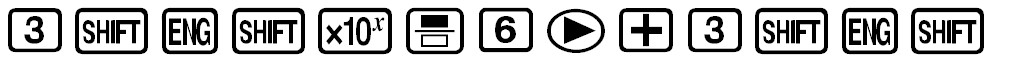
\includegraphics[width=0.5\textwidth]{../figs/VN12-PH-06-A-004-1-V2-8.jpg}
			\end{center}
			
			\begin{center}
				
\includegraphics[width=0.5\textwidth]{../figs/VN12-PH-06-A-004-1-V2-9.jpg}
			\end{center}
		\end{description} 
		
		Ta thu được kết quả hiển thị trên màn hình là biên độ  $A=3\sqrt{3}\text{cm}$, pha ban đầu $\varphi=\dfrac{\pi}{3}\ \text{rad}$ của dao động tổng tổng hợp.
		
		Vậy $x=3\sqrt{3}\cos\left(4\pi t+\dfrac{\pi}{3}\right) \textrm{cm}$.
		
		\textbf{Đáp án: A.}
	}
	\viduii{3}{Hai dao động cùng phương lần lượt có phương trình $x_1 = A_1\cos \left(\pi t + \dfrac{\pi}{6}\right)\ \text{cm}$ và\\ $x_2 = 6 \cos \left(\pi t - \dfrac{\pi}{2}\right)\ \text{cm}$. Dao động tổng hợp của hai dao động này có phương trình $x = 10 \cos(\omega t + \varphi)$. Thay đổi $A_1$ đến khi biên độ $A$ đạt giá trị cực tiểu. Khi đó giá trị của $\varphi$ là
		\begin{mcq}(4)
			\item $ - \dfrac{\pi}{6}$.
			\item $ - \dfrac{\pi}{3}$.
			\item $ \pi $.
			\item $0$.
		\end{mcq}
	}
	{\begin{center}
			\textbf{Hướng dẫn giải}
		\end{center}
		
		Biên độ dao động tổng hợp $$A^2 = A_1^2+6^2 + 2A_16 \cos \dfrac{2\pi}{3}.$$
		
		Để $A$ nhỏ nhất thì
		$A_1 = - \dfrac{2 \cdot 6 \cos \dfrac{2\pi}{3}}{2}=3\ \text{cm}.$
		
		Khi đó:
		\begin{equation*}\label{eq2}
			\tan\varphi = 	\dfrac{A_1\sin\varphi_1+A_2\sin\varphi_2}		{A_1\cos\varphi_1+A_2\cos\varphi_2} = -\sqrt 3 \Rightarrow \varphi =- \dfrac{\pi}{3}. 
		\end{equation*}
		\textbf{Đáp án: B.}
	}
	
\end{dang}
